\documentclass{article}

% Packages
\usepackage[utf8]{inputenc} % UTF-8 input encoding
\usepackage[T1]{fontenc} % Font encoding
\usepackage{amsmath, amssymb} % Math packages
\usepackage{enumitem} % For customizing lists
\usepackage{lipsum} % For generating dummy text
\usepackage{listings}
\usepackage{graphicx}


\lstset{%
  language=bash,
  basicstyle=\fontfamily{pcr}\selectfont,
  commentstyle=\bfseries,
  escapeinside={(*@}{@*)}
}

\newcommand{\comment}[1]{\# here is a comment: #1}
\newcommand\floor[1]{\lfloor#1\rfloor}
\newcommand\ceil[1]{\lceil#1\rceil}

% Title and author information
\title{Evolutionary Computation (6560) HW01}
\author{Alex Darwiche}
\date{\today}

\begin{document}

\maketitle

\section*{Answers}

% Question 1
\subsection*{Q1: Subset Problem}
\begin{enumerate}[label=(\alph*)]
    \item \textbf{Representation:}
    \subitem (1) Binary Vector of Length N
    \subitem (2) 0 means not in Subset P
    \subitem (3) 1 mean in Subset P

    \item \textbf{Fitness Function:}
    \subitem (1) Distance from 21, to be minimized.
    \subitem (2) Or the abolsute value of sum of all elements in P, minus 21.
    \subitem (3) Fitness Formula = Min($|\sum p - 21|$)
    \subitem (4) 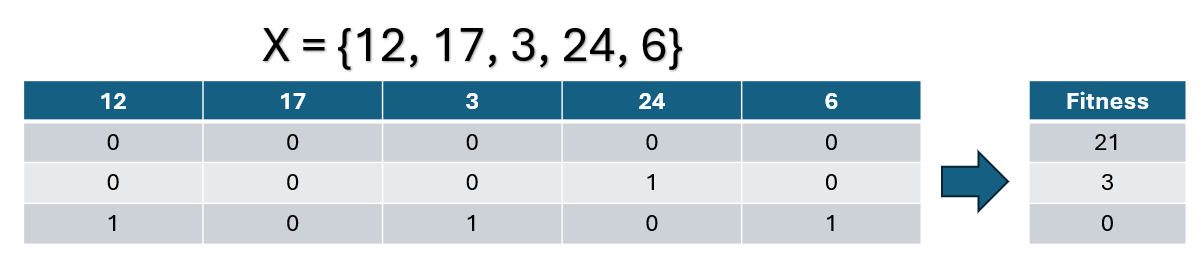
\includegraphics[width=.75\textwidth]{fitness_problem1.PNG}

    \item \textbf{Mutation:}
    \subitem (1) Bit-Flip Mutation with probability 1/N

    \item \textbf{Crossover:}
    \subitem (1) 1-point crossover between two parents

    \item \textbf{Repair:}
    \subitem (1) If the $\sum p > 21$ then flip a random 1 to 0.
    \subitem (2) If the $\sum p < 21$ then flip a random 0 to 1.
    \subitem (3) Computationally Heavy Option: Calculate the distance from 21 of $\sum p$, and only swap lowest value that is less than the distance from either 0 to 1 or 1 to 0, depending on if $\sum p$ > 21 or < 21.
    

    \item \textbf{Termination:}
    \subitem (1) Fitness = 0 or reach 10,000 steps.
\end{enumerate}

% Question 2
\subsection*{Q2: Graph K-colording Problem}
\begin{enumerate}[label=(\alph*)]
    \item \textbf{Representation:}
    \subitem (1) Integer Representation Vector of Length N
    \subitem (2) Each integer corresponds to a color from 1 to k
    \subitem (3) 0 means Red
    \subitem (4) 1 means Blue
    \subitem (5) \dots
    \subitem (6) k means k-th color

    \item \textbf{Fitness Function:}
    \subitem (1) Minimize the number of conflicted edges. 
    \subitem (2) A conflicted edge is one that has the same color on each vertex.
    \subitem (3) Fitness Formula = Min(Count(Conflicted Edges of E))
    \subitem (3) 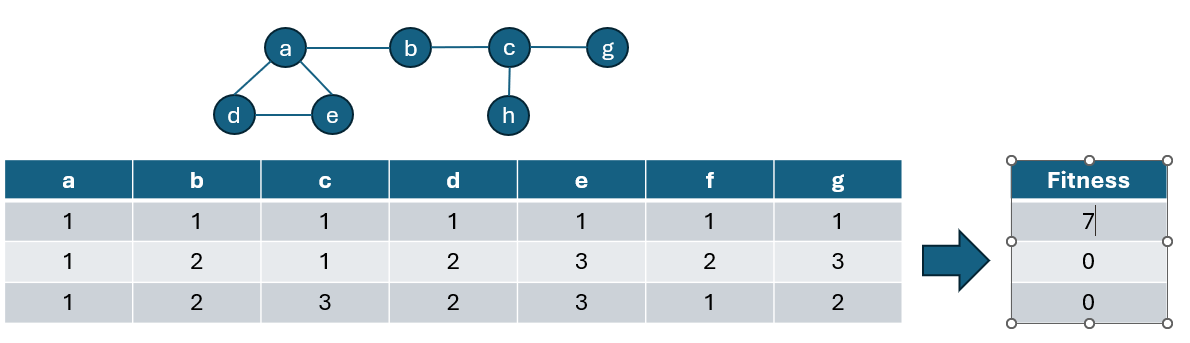
\includegraphics[width=.75\textwidth]{fitness_problem2.PNG}

    \item \textbf{Mutation:}
    \subitem (1) Flip Mutation with probability 1/N, changing to one of (K-1) other color options

    \item \textbf{Crossover:}
    \subitem (1) 1-point crossover between two parents

    \item \textbf{Repair:}
    \subitem (1) If a conflicted edge exists, change the color of the edge with the least amount of neighbors to a random different color.    

    \item \textbf{Termination:}
    \subitem (1) Fitness = 0 or reach 10,000 steps.
\end{enumerate}

% Question 3
\subsection*{Q3: Minimum Vertex Cover}
\begin{enumerate}[label=(\alph*)]
    \item \textbf{Representation:}
    \subitem (1) Binary Vector of Length N
    \subitem (2) 0 means not in X
    \subitem (3) 1 mean in X

    \item \textbf{Fitness Function:}
    \subitem (1) Maximize (N*Good edges) + (N-Size of X).
    \subitem (2) Good Edges: This is an edge that is only touched by only 1 vertex in X. We multiply it by N to ensure finding good edges is the first priority, then the second term helps to ensure we find the minimum vertex cover among feasible options.
    \subitem (3) Bad Edges: This is an edge that is touched by 2 or 0 vertices in X.
    \subitem (4) (N-Size of X): This incentivizes finding a smaller solution set.
    \subitem (3) 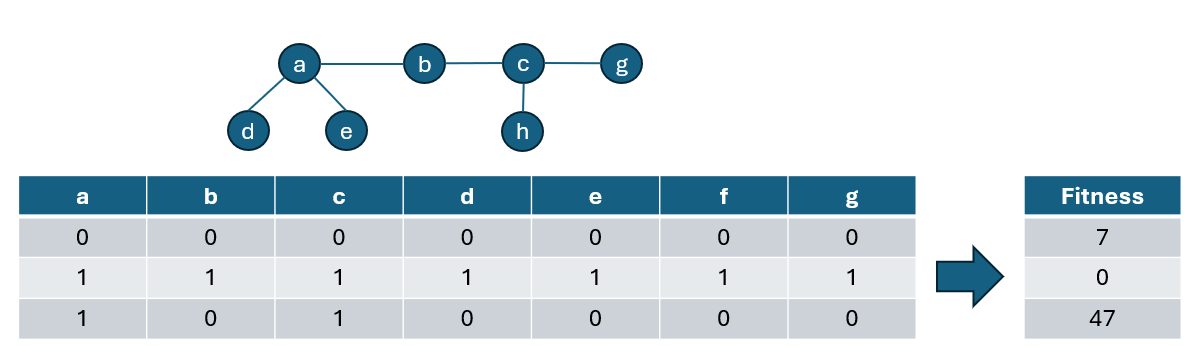
\includegraphics[width=.75\textwidth]{fitness_problem3.PNG}

    \item \textbf{Mutation:}
    \subitem (1) Bit-Flip Mutation with probability 1/N

    \item \textbf{Crossover:}
    \subitem (1) 1-point crossover between two parents

    \item \textbf{Repair:}
    \subitem (1) Swap the value of a vertex if it is part of a "bad" edge. This can be either changing from 1 to 0 or 0 to 1 depending on if the edge is bad because it is touched by no vertex in X, or if its touched by 2 vertices in X.

    \item \textbf{Termination:}
    \subitem (1) Fitness = (N*M + N) or Reach 10,000 steps.
    \subitem (2) (N*M + (N-1)) is the maximum possible value of fitness. Essentially all edges are good AND only 1 vertex is used in the cover. This assumes that there exists at least 1 edge.
\end{enumerate}

\end{document}
